
%% Formato para la presentaci\'on de  proyectos de grado. 
%% Maestría en Ingeniería de Software
%% Pontificia Universidad Javeriana
%% Elaborado por Angela Villota y Luisa Rincón
%% Inspirado en Formato elaborado para carrera de Ing de Sistemas
%% V 1.0 Abril - 2022
\documentclass[12pt]{article}
\usepackage[utf8]{inputenc}
\usepackage{geometry}
\geometry{letterpaper}
\usepackage[spanish,es-tabla]{babel}
% \usepackage{cite}
\usepackage{titling}
\usepackage{setspace}
\usepackage{graphicx}
\graphicspath{{img/}} %ruta de la carpeta en donde estaràn las imágenes
\usepackage{blindtext}
\usepackage[hidelinks]{hyperref}
\setlength{\marginparwidth}{2cm}
\usepackage{natbib} %% para citaciones
\usepackage{todonotes}
\usepackage[format=hang,font=small,labelfont=bf]{caption}

\usepackage{pgfgantt}
\usepackage{lscape}
\usepackage{rotating}

\usepackage{enumitem}

% *** ALIGNMENT PACKAGES ***
%
\usepackage{array}
\usepackage{booktabs}
\usepackage{pdflscape}
\usepackage{multirow}
\usepackage{float}
\usepackage{longtable}
\usepackage{dblfloatfix}
\usepackage{subfig}

\onehalfspacing
\setcounter{secnumdepth}{5}
\setcounter{tocdepth}{2}

\usepackage{xcolor}
\definecolor{light-gray}{gray}{0.95}
\newcommand{\code}[1]{\colorbox{light-gray}{\texttt{#1}}}

\renewcommand\maketitlehooka{\null\mbox{}\vfill}
\renewcommand\maketitlehookd{\vfill\null}
\DeclareUnicodeCharacter{0301}{\hspace{-1ex}\'{ }}

\begin{document}
%crear titulo
%\maketitle

%%%%%%%%%%%%%%%%%
% Portada del Anteproyecto
%%%%%%%%%%%%%%%%%
\begin{center}
\thispagestyle{empty}
\vspace*{-2cm}
\begin{center}
    
\includegraphics[width=9cm]{pujlogo}~\\[1cm]
\end{center}
\textbf{\huge
Marco de trabajo para implementación de buenas prácticas y directrices para la integración de nuevos productos con Inteligencia Artificial en las arquitecturas existentes}\\[1.3cm]
% T\'{\i}tulo de la tesis  o trabajo de investigación}\\[1.75cm]
\Large\textbf{Fabian Andres Caicedo Cuellar}\\[1cm]
\small Anteproyecto presentada(o) como requisito parcial para optar al
t\'{\i}tulo de:\\
\textbf{Magister en Ingenier\'{\i}a de Software}\\[1cm]
Director(a):\\
T\'{\i}tulo (Ph.D., MSc) y nombre del director(a)\\[1.4cm]

Pontificia Universidad Javeriana Cali\\
Facultad de Ingeniería\\
Departamento de Electrónica y Ciencias de la Computación\\
Cali, Colombia\\
\today\\
\end{center}

\newpage
%%%%%%%%%%%%%%%%%
% Ficha resumen
%%%%%%%%%%%%%%%%%
\thispagestyle{empty}
\begin{center}
    \Large{Ficha Resumen \\ Anteproyecto de Trabajo de Grado}
\end{center}

\textbf{Marco de trabajo para la integración de herramientas de IA en los productos de software para el área de Seguridad y Salud en el Trabajo desarrollados por la Corporación Talentum}
\begin{enumerate}
    \item Área de trabajo: Ingeniería y tecnología
    \item Tipo de proyecto: Aplicado
    \item Estudiante: Fabián Andrés Caicedo Cuellar
    \item Correo electrónico: fabiancaicedo@javerianacali.edu.co
    \item Dirección y teléfono: Carrera 23C \#10-02 / 3176367317
    \item Director: Oscar Orlando Ceballos Argote, Ph.D.
    \item Vinculación del director: Hora C\'atedra
    \item Correo electrónico del director: oscar.ceballos@javerianacali.edu.co
    %\item Co-Director (Si aplica):
    \item Grupo o empresa que lo avala (Si aplica): Corporación Talentum
    % \item Otros grupos o empresas:
    \item Palabras clave(al menos 5): Inteligencia Artificial (IA), Seguridad y Salud en el Trabajo
(SST), Ingeniería de Software (IS).
    \item Fecha de inicio: 1 de Enero de 2024
    \item Duración estimada (en meses): 6 meses
    \item Resumen:  La propuesta de investigación presentada propone un marco de trabajo integral y detallado para la incorporación efectiva de componentes basados en Inteligencia Artificial (IA) en arquitecturas de software ya existentes, poniendo especial atención en el ámbito de la seguridad y salud laboral. Mediante un análisis y revisión de la literatura existente, se examina la problemática asociada a la integración de la IA en sistemas preexistentes, identificando así los retos técnicos, arquitectónicos y contextuales que implica la implementación de esta tecnología.

En este marco, se utiliza como caso de estudio la Corporación Talentum, una entidad prominente en la implementación de proyectos gubernamentales en Colombia. Esta corporación afronta desafíos significativos para integrar productos de IA en sus soluciones, resaltando la urgente necesidad de establecer un conjunto estandarizado de buenas prácticas y directrices.

La propuesta de investigación propone un marco de trabajo que comprende una serie de buenas prácticas, componentes arquitectónicos potenciales y criterios específicos destinados a lograr una integración efectiva de la IA. El objetivo de este marco no es únicamente facilitar la adaptación técnica, sino también maximizar los beneficios derivados de la IA, asegurando así su relevancia y sostenibilidad a largo plazo. Como parte de la propuesta, se presenta un prototipo funcional web y modular, que sirve como caso práctico para validar la aplicabilidad del marco de trabajo propuesto.

Se anticipa que los resultados de este trabajo incluyan un documento que defina el marco de trabajo y proporcione buenas prácticas para la integración de la IA, acompañado de un conjunto de diagramas UML y del modelo C4 para ilustrar los componentes arquitectónicos sugeridos. Se espera, además, que el prototipo funcional demuestre de manera tangible la utilidad y aplicabilidad del marco de trabajo en contextos reales.

Este trabajo aporta significativamente al campo de la IA y la arquitectura de software, ofreciendo una guía práctica y un conjunto de herramientas útiles para la integración de productos basados en IA en soluciones ya existentes. De igual manera, subraya la necesidad de una implementación orientada de la IA, especialmente en sectores de crítica importancia como lo es la seguridad y salud en el trabajo.

\end{enumerate}

\newpage

%%%%%%%%%%%%%%%%%
% Indices y tablas
%%%%%%%%%%%%%%%%%

\tableofcontents
\listoffigures
\listoftables
% \listoftodos
\newpage

%%%%%%%%%%%%%%%%%
% Resumen / abstract
%%%%%%%%%%%%%%%%%
%%%%%%%%%%%%%%%%
% ABSTRACT
%%%%%%%%%%%%%%%%

\section*{Resumen}
A pesar de los evidentes avances en el área de la Inteligencia Artificial (IA), su integración efectiva en soluciones de software orientadas a la Seguridad y Salud en el Trabajo (SST) presenta desafíos que abarcan desde aspectos técnicos hasta cuestiones éticas y de privacidad, y demandan una comprensión profunda y enfoques adaptados para asegurar implementaciones exitosas que realmente beneficien a los usuarios finales y a las organizaciones involucradas.

De ahí que, la presente propuesta de investigación propone un marco de trabajo para incorporar componentes de IA en arquitecturas de software preexistentes con énfasis en SST. El marco de trabajo se compone de prácticas recomendadas, componentes arquitectónicos y criterios para una integración eficaz de una IA, buscando no solo la adaptación técnica sino también el aprovechamiento máximo de la IA para garantizar su impacto y perdurabilidad. 

En particular, como caso de estudio, se seleccionará un proyecto de desarrollo de software el cual incluya en sus requerimientos funcionales la necesidad de incorporar componentes de IA. La Corporacion Talentum es una entidad prominente en la implementaci on de proyectos gubernamentales en Colombia.

%Los resultados esperados son un manual de buenas prácticas, diagramas UML, y el modelo C4, junto con un prototipo que evidencie la funcionalidad del marco en situaciones reales. Este trabajo contribuye al campo de IA y arquitectura de software, proveyendo guías y herramientas para la integración de IA, resaltando la importancia de una implementación orientada y consciente en ámbitos críticos como la seguridad y salud laboral.


% La propuesta de investigaci\'on presentada propone un marco de trabajo integral y detallado para la incorporación efectiva de componentes basados en Inteligencia Artificial (IA) en arquitecturas de software ya existentes, poniendo especial atención en el ámbito de la seguridad y salud laboral. Mediante un análisis y revisión de la literatura existente, se examina la problemática asociada a la integración de la IA en sistemas preexistentes, identificando así los retos técnicos, arquitectónicos y contextuales que implica la implementación de esta tecnología.

% En este marco, se utiliza como caso de estudio la Corporación Talentum, una entidad prominente en la implementación de proyectos gubernamentales en Colombia. Esta corporación afronta desafíos significativos para integrar productos de IA en sus soluciones, resaltando la urgente necesidad de establecer un conjunto estandarizado de buenas prácticas y directrices.

% La propuesta de investigaci\'on propone un marco de trabajo que comprende una serie de buenas prácticas, componentes arquitectónicos potenciales y criterios específicos destinados a lograr una integración efectiva de la IA. El objetivo de este marco no es únicamente facilitar la adaptación técnica, sino también maximizar los beneficios derivados de la IA, asegurando así su relevancia y sostenibilidad a largo plazo. Como parte de la propuesta, se presenta un prototipo funcional web y modular, que sirve como caso práctico para validar la aplicabilidad del marco de trabajo propuesto.

% Se anticipa que los resultados de este trabajo incluyan un documento que defina el marco de trabajo y proporcione buenas prácticas para la integración de la IA, acompañado de un conjunto de diagramas UML y del modelo C4 para ilustrar los componentes arquitectónicos sugeridos. Se espera, además, que el prototipo funcional demuestre de manera tangible la utilidad y aplicabilidad del marco de trabajo en contextos reales.

% Este trabajo aporta significativamente al campo de la IA y la arquitectura de software, ofreciendo una guía práctica y un conjunto de herramientas útiles para la integración de productos basados en IA en soluciones ya existentes. De igual manera, subraya la necesidad de una implementación orientada de la IA, especialmente en sectores de crítica importancia como lo es la seguridad y salud en el trabajo.




\paragraph*{}{\textbf{Palabras Clave:}}
Inteligencia Artificial (IA), Seguridad y Salud en el Trabajo (SST), Ingenier\'ia de Software (IS), Marco de Trabajo, Prompt.

\section*{Abstract}
Despite the evident advances in the area of Artificial Intelligence (AI), its effective integration into software solutions focused on Occupational Health and Safety (OSH) presents challenges that range from technical aspects to ethical and privacy issues and demand deep understanding and tailored approaches to ensure successful implementations that truly benefit end users and the organizations involved.

Hence, the present research proposal proposes a framework to incorporate AI components into pre-existing software architectures with an emphasis on SST. The framework is made up of recommended practices, architectural components and criteria for an effective integration of an AI, seeking not only technical adaptation but also the maximum use of AI to guarantee its impact and durability.

In particular, as a case study, a software development project will be selected which includes in its functional requirements, the need to incorporate AI components. The Talentum Corporation is a
Prominent entity in the implementation of government projects in
Colombia.


%This research proposal comprises a framework for incorporating Artificial Intelligence (AI) into pre-existing software architectures, with an emphasis on occupational health and safety. It analyzes the challenges of integrating AI into established software systems, covering technical, structural and contextual issues. The central case study is the Talentum Corporation in Colombia, highlighting the need for standardized practices for AI insertion in government projects.

%The proposed framework consists of best practices, architectural components and criteria for effective AI integration, seeking not only technical adaptation but also the maximum use of AI to ensure its impact and durability. It includes a modular web prototype to validate its feasibility.

%The expected results are a best practices manual, UML diagrams, and the C4 model, along with a prototype that evidences the functionality of the framework in real situations. This work contributes to the field of AI and software architecture, providing guidelines and tools for AI integration, highlighting the importance of a targeted and conscious implementation in critical areas such as occupational health and safety.

\paragraph*{}{\textbf{Keywords:}}
Artificial Intelligence (AI), Occupational Safety and Health (OSH), Software Engineering (SE), Framework, Prompt. 
\newpage

%%%%%%%%%%%%%%%%%
% Introduccion
%%%%%%%%%%%%%%%%%
\section{Introducción}

Aquí algunos ejemplos de como se usan las imágenes, las tablas las listas

\textbf{ text in bold}
\textit{text in italics}
\underline{underlined text}
\texttt{text in consola-like font}

\subsection*{Ejemplos de listas}
itemize, enumerate, description

\begin{itemize}
    \item cada item es una viñeta
    \item Otra viñeta
\end{itemize}

\begin{enumerate}
    \item enumeración
    \begin{enumerate}
        \item anidado
    \end{enumerate}
\end{enumerate}

\begin{figure*}[htb]
\centering
\subfloat[] {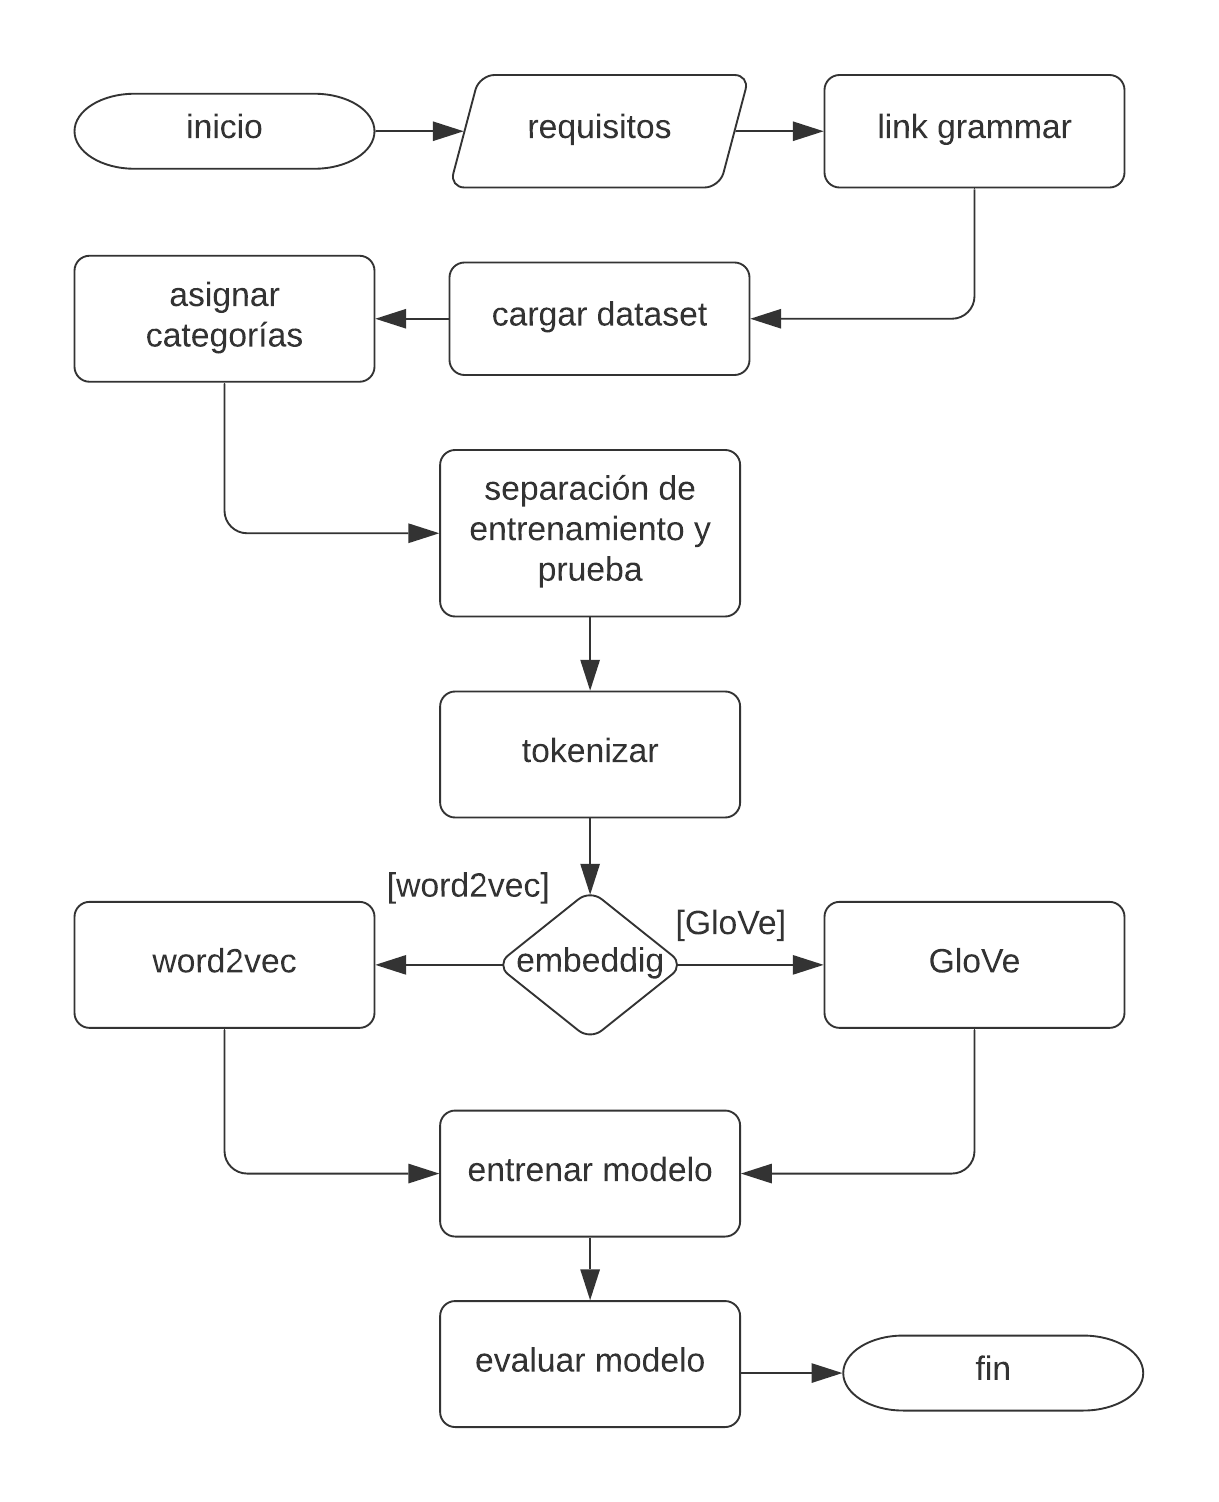
\includegraphics[width=0.4\textwidth]{Deep.png}

\label{fig:PAS_FM}}
\subfloat []{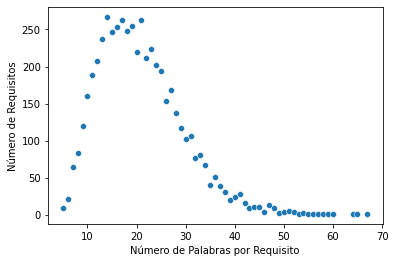
\includegraphics[width=0.38\textwidth]{freq_req.png}

\label{fig:PAS_FM2}}

\label{fig:examples}
\end{figure*}
 
 \begin{table}[htb]
     \centering
     \begin{tabular}{rc}
	\toprule
    	Item1 & Item2  \\
	\midrule
	celda 1 & celda 2\\
 celda 3 & celda 4\\
	\bottomrule

\end{tabular}
     \caption{Propuesta de elementos identificados en el desarrollo del proyecto. Fuente \citep{Hinton2012}}
     \label{tab:my_label}
 \end{table}

\subsection*{Uso de figuras}
La Figura \ref{fig:figure1} muestra un gráfico de ejemplo. Las tablas y figuras que aparecen en el documento deben ser previamente introducidas y explicadas \todo{algo}


\begin{figure}
\centering
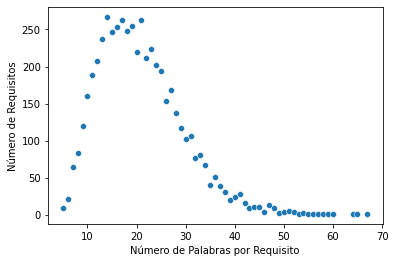
\includegraphics[width=0.5\textwidth]{freq_req.png}
\caption{Grafico tridimensional. Elaboración propia}
\label{fig:figure1}
\end{figure} 
\newpage

%% Problema
\section{Definición del problema}

\subsection{Planteamiento del problema}
En la era digital actual, la Inteligencia Artificial (IA) ha transformado rápidamente múltiples sectores, se puede decir que desde la atención médica y la manufactura hasta el entretenimiento y la logística. Su virtud para analizar gran cantidad o volúmenes de datos, hacer predicciones precisas y automatizar tareas complejas ha demostrado ser un activo invaluable. Dentro del campo del desarrollo y la arquitectura de software, la integración de la IA presenta oportunidades únicas para mejorar la eficiencia, la funcionalidad y la experiencia del usuario.

No obstante, mientras muchas organizaciones están ansiosas por adoptar y beneficiarse de las capacidades de la IA, enfrentan desafíos significativos. Uno de los principales desafíos es la falta de un conjunto estandarizado de buenas prácticas que guíen la integración de soluciones de IA en arquitecturas de software preexistentes \citep{Wang2016ImplementingOutlook}. Esta ausencia puede dar lugar a incompatibilidades, redundancias, ineficiencias y, en el peor de los casos, a fallas en el sistema.

La integración eficiente y efectiva de productos basados en IA en sistemas existentes es esencial para mantener la relevancia en un mercado en constante cambio y para aprovechar al máximo los beneficios o ventajas que ofrece la IA. Esta integración no solo implica la adaptación técnica, sino también la consideración de cómo los productos de IA pueden añadir valor real a los usuarios y a la organización \citep{Cui2022ConstructionIntelligence}. Sin una orientación clara y prácticas estandarizadas, las organizaciones pueden encontrarse con sistemas sobre complicados, costosos y que no cumplen con las expectativas.

Por otra parte, aunque la literatura ha abordado ampliamente las capacidades y aplicaciones de la IA, existe una notoria falta de investigación exhaustiva sobre la estrategia de integración de estas soluciones en el mercado tecnológico \citep{Cui2022ConstructionIntelligence}. Esta laguna en la investigación puede dificultar a las organizaciones la toma de decisiones informadas sobre cómo abordar la integración de IA.

Adicionalmente, con la rápida evolución del mercado y la tecnología, las organizaciones se ven presionadas a adaptarse rápidamente a las necesidades cambiantes \citep{Wang2016ImplementingOutlook}. Sin un marco de referencia sólido, esta adaptación puede volverse reactiva en lugar de proactiva, lo que puede llevar a soluciones temporales o inadecuadas.

En el contexto colombiano, la Corporación Talentum ha consolidado una sólida reputación como ejecutora de proyectos gubernamentales, tanto tecnológicos como no tecnológicos. Estos proyectos, destinados a generar un alto impacto en diferentes sectores gubernamentales, resaltan la importancia de la seguridad y salud en el trabajo. El objetivo primordial de la corporación es mejorar sus procesos de seguridad y salud en el trabajo. No obstante, la Corporación Talentum aspira a ejecutar proyectos gubernamentales con productos propios que incorporen Inteligencia Artificial. La intención es respaldar y ofrecer mejoras en los procesos de estas entidades, creyendo que, al hacerlo, indirectamente contribuirán a mejorar las condiciones y el ambiente laboral. Al promover el bienestar de los empleados a través de estas iniciativas, la corporación manifiesta su compromiso con la salud laboral en Colombia.

A lo largo de su trayectoria, la Corporación Talentum ha reconocido la trascendencia de la Inteligencia Artificial en la configuración de soluciones de vanguardia. Sin embargo, enfrenta desafíos considerables en su intento de incorporar productos de IA, acentuando la sensación de quedar rezagados frente a otras entidades que ya han adoptado estas tecnologías como parte integral de sus ofertas. Esta situación no solo se traduce en una potencial desventaja competitiva, sino que también refleja un desaprovechamiento de oportunidades para aportar valor innovador en el sector de seguridad y salud en el trabajo. La falta de un marco de trabajo adecuado para la integración de la Inteligencia Artificial ha supuesto un desafío para la Corporación Talentum, lo cual podría influir negativamente en su posicionamiento como ejecutora líder de proyectos gubernamentales en Colombia.

Por lo tanto, se hace imperativo investigar y desarrollar un marco de trabajo que proporcione un conjunto de directrices base y mejores prácticas para la integración de productos basados en IA en arquitecturas de software existentes. Esta necesidad no solo es esencial para maximizar los beneficios de la IA, sino también para garantizar la viabilidad, la escalabilidad y la relevancia a largo plazo de las soluciones tecnológicas cada vez más orientado hacia la IA.

\subsection{Formulación del problema}

En la actualidad, la influencia creciente de la inteligencia artificial (IA) en el desarrollo de software exige que las organizaciones, incluida la Corporación Talentum en Colombia, adapten sus estrategias para mantener su competitividad. A pesar de reconocer el potencial de la IA en el sector de seguridad y salud en el trabajo, la corporación enfrenta desafíos en su incorporación debido a la falta de directrices claras y una estrategia bien definida.
Dado el panorama actual de las empresas que desarrollan software y teniendo en cuenta las particularidades y objetivos de la Corporación Talentum, surgen las siguientes interrogantes enfocadas en el sector de seguridad y salud en el trabajo:
\begin{itemize}
    \item ¿Cómo pueden las soluciones orientadas al sector de seguridad y salud en el trabajo incorporar efectivamente componentes de inteligencia artificial en los requerimientos funcionales del software?
    \item ¿Qué buenas prácticas, estándares y componentes arquitectónicos se deben adoptar para facilitar la integración de productos basados en IA en arquitecturas de software preexistentes?
    \item ¿De qué manera se asegura que la integración de IA en las soluciones de software no solo aporte beneficios técnicos y funcionales, sino que también respete los principios éticos del sector de seguridad y salud en el trabajo?
    \item ¿Qué consideraciones arquitectónicas son necesarias para gestionar adecuadamente los prompts de Inteligencia Artificial, asegurando una comunicación eficiente y precisa con sistemas preexistentes?
\end{itemize}

Con estas preguntas, se busca abordar la problemática central relacionada con la integración eficiente de la IA en las soluciones de software de la Corporación Talentum en el ámbito de la seguridad y salud en el trabajo. El objetivo es identificar áreas clave de desafío y establecer una estructura que guíe la investigación y desarrollo de directrices y mejores prácticas para este proyecto de maestría.
\newpage

%% Objetivos
\section{Objetivos del proyecto}
\subsection{Objetivo General}
 Proponer un marco de trabajo que guíe la integración de componentes de Inteligencia Artificial en soluciones de software orientadas al sector de Seguridad y Salud en el Trabajo con base en los requerimientos funcionales.

%Definir buenas prácticas y estrategias para la incorporación de componentes de Inteligencia Artificial en soluciones software orientadas al sector de Seguridad y Salud en el Trabajo.

\subsection{Objetivos específicos}
\begin{enumerate}[label=\textbf{OE\arabic*:}]
    \item Elaborar una lista de buenas prácticas para la incorporación de funcionalidades de Inteligencia Artificial en arquitecturas de productos de software específicos para el sector de Seguridad y Salud en el Trabajo.
    \item Proponer una lista de componentes arquitectónicos potenciales para considerar en la integración de Inteligencia Artificial dentro del desarrollo de soluciones de software.
    \item Definir un conjunto de criterios que permitan especificar el contexto necesario para que la Inteligencia Artificial proporcione respuestas de manera más precisa, enfocándose especialmente en la elaboración y gestión de prompts.
    \item Identificar y proponer posibles adaptaciones arquitectónicas necesarias para la integración de componentes de Inteligencia Artificial en arquitecturas preexistentes de soluciones de software en el ámbito de la seguridad y salud laboral.
\end{enumerate}


\subsection{Resultados esperados}

\begin{enumerate}[label=\textbf{R\arabic*}]
    \item \textbf{(OE1):} Lista de buenas prácticas en la integración de IA en productos de software se enfoca en una gestión de recursos computacionales, la elección de herramientas o librerías optimizadas para la tarea y la selección de modelos de IA específicos para la industria. Este conjunto de prácticas se basa en el análisis de las necesidades computacionales del software para asignar recursos de manera eficiente, la evaluación de herramientas y librerías por su compatibilidad, rendimiento y soporte comunitario, y la elección de modelos de IA que no solo estén en la vanguardia tecnológica, sino que también se alineen estrechamente con los objetivos y procesos industriales específicos del producto.
    \item \textbf{(OE2):} Lista de componentes arquitectónicos para integrar IA durante la fase de diseño de software es una guía para identificar cada elemento necesario y su función dentro del sistema, incluyendo las entradas y salidas de información. Se requiere una comprensión de cómo cada componente interactúa con el sistema existente y cómo el flujo de datos entre estos componentes impulsa las operaciones de IA. Esto ayuda a los diseñadores y desarrolladores a establecer fronteras de responsabilidad y a garantizar que todos los elementos de la arquitectura estén sincronizados para el rendimiento óptimo del sistema.
    \item \textbf{(OE3):} Lista de criterios enfocados en Seguridad y Salud en el Trabajo para configurar adecuadamente el contexto al formular preguntas a un componente de IA, lo que resulta en respuestas más precisas y pertinentes. Estos criterios deben abordar aspectos específicos como la naturaleza del entorno laboral, los riesgos potenciales y las normativas de seguridad aplicables. Al integrar estos elementos en los prompts, la IA puede ajustar sus respuestas para ofrecer información que no solo sea correcta sino también aplicable y segura según las directrices de SST del contexto en cuestión.
    \item \textbf{(OE4):} Lista de posibles adaptaciones arquitectónicas en arquitecturas de software preexistentes para la incorporación de IA aborda la expansión de la capacidad de cómputo, la mejora o adición de interfaces para la integración de nuevos componentes de IA y la actualización de dependencias obsoletas. Estas adaptaciones son fundamentales para superar los desafíos más comunes y para facilitar la transición hacia sistemas mejorados con inteligencia artificial, garantizando que la arquitectura existente se mantenga relevante y pueda soportar las nuevas cargas de trabajo y funcionalidades.
    \item \textbf{(OE4):} Lista de recomendaciones para la modificación o ampliación de arquitecturas de software existentes toma en cuenta las peculiaridades inherentes a los diferentes estilos arquitectónicos en la integración de la IA. Estos estilos incluyen arquitecturas monolíticas, microservicios y basada en servicios, proporcionando una guía para incorporar componentes de IA en el desarrollo evolutivo del software.
\end{enumerate}


% \begin{enumerate}
%     \item Un documento que establece un marco de trabajo, incluyendo prácticas recomendadas para integrar funcionalidades de Inteligencia Artificial en arquitecturas de productos de software, posibles criterios para definir el contexto necesario que permita a la Inteligencia Artificial proporcionar respuestas más precisas, y guías para realizar adaptaciones arquitectónicas en soluciones de software preexistentes.
%     \item Un conjunto de diagramas UML y diagramas del modelo C4, extendiéndose hasta el nivel de componentes, para ilustrar los componentes potenciales a considerar en la integración de Inteligencia Artificial en el desarrollo de soluciones de software. Todos estos diagramas se integrarán y explicarán dentro del marco de trabajo.
%     \item Desarrollo de un prototipo funcional implementado en una plataforma web modular como caso de estudio para validar la propuesta del marco de trabajo.% que sirva para demostrar la aplicación práctica del marco de trabajo desarrollado, facilitando la integración de componentes de Inteligencia Artificial y funcionando 
% \end{enumerate}
\newpage

%% Alcance
\section{Alcance}
El presente proyecto se centra en la integración de componentes de Inteligencia Artificial (IA) en soluciones de software específicas para el sector de Seguridad y Salud en el Trabajo (SST). Se busca comprender las funcionalidades y características de los sistemas de software actuales en este sector, identificando áreas de oportunidad donde la IA pueda potenciar o mejorar dichas funcionalidades.

Es importante dentro del alcance de este trabajo la creación de un compendio de buenas prácticas para la incorporación de funcionalidades de IA, esperando que sirva de guía para futuras implementaciones. De forma complementaria, se propondrá una lista de componentes arquitectónicos que podrían considerarse en la integración de la IA dentro de las soluciones de software ya existentes.

Se definirán criterios específicos para asegurar que la IA entregue respuestas precisas y relevantes, con especial atención en la elaboración y gestión del contexto que requieren los prompts enfocados en SST. Además, se identificarán y propondrán las adaptaciones arquitectónicas necesarias en las arquitecturas de software preexistentes para facilitar la integración de la IA, lo cual es esencial para una incorporación exitosa y eficiente.

Para validar la propuesta del marco de trabajo, se desarrollará un prototipo funcional implementado en una plataforma web modular. Sin embargo, es importante señalar lo que este proyecto no abarcará:
\begin{itemize}
    \item No se desarrollarán nuevos componentes de IA desde cero; en su lugar, se utilizarán modelos ya existentes para lograr la interoperabilidad con las soluciones de software actuales.
    \item Solo se examinarán tres estilos arquitectónicos: arquitecturas monolíticas, microservicios y basadas en servicios, excluyendo cualquier otro estilo arquitectónico.
    \item Las buenas prácticas que se revisarán estarán únicamente enfocadas en la gestión de recursos computacionales, la selección de herramientas o librerías y modelos de IA pertinentes, sin extenderse a otras áreas de práctica que puedan influir en la integración de la IA.
    \item Este trabajo se centrará predominantemente en la fase de diseño del desarrollo de software, particularmente en lo que respecta a la arquitectura de software, sin abarcar las fases posteriores de implementación y mantenimiento.
\end{itemize}

La adopción de este enfoque selectivo asegura que el proyecto se desarrolle dentro de un marco delimitado, lo que facilitará la consecución de los objetivos propuestos, asegurándose de que sean prácticos y realistas. Estableciendo estas limitaciones de manera explícita, se configura un contorno para el trabajo de investigación, lo cual contribuirá significativamente al ámbito de SST. Así, el documento resultante no solo reflejará una investigación dirigida y metódica, sino que también se espera que sea una contribución valiosa, ofreciendo perspectivas y soluciones aplicables al sector específico de SST.







% El alcance de este proyecto se centra en la integración de componentes de Inteligencia Artificial (IA) en soluciones de software específicas para el sector de seguridad y salud en el trabajo. Se busca comprender a fondo las funcionalidades y características de los sistemas de software actuales en este sector, identificando áreas de oportunidad donde la IA pueda potenciar o mejorar dichas funcionalidades.

% La elaboración de una lista de buenas prácticas para la incorporación de funcionalidades de IA es un aspecto importante de este proyecto, y se espera que sirva como guía para futuras implementaciones. Paralelamente, se propondrá una lista de componentes arquitectónicos potenciales que podrían ser considerados en la integración de IA dentro de soluciones de software existentes.

% El trabajo también implica la definición de criterios específicos para garantizar que la IA proporcione respuestas precisas y relevantes, con un enfoque particular en la elaboración y gestión de prompts. Esto es fundamental para mejorar la efectividad de las soluciones propuestas y evitar malentendidos o inexactitudes en las respuestas de la IA.

% En cuanto a las adaptaciones arquitectónicas, este proyecto identificará y propondrá cambios necesarios en las arquitecturas de software preexistentes para facilitar la integración de componentes de IA. Este aspecto es vital para asegurar una integración óptima y eficiente, aprovechando al máximo las capacidades de la IA.

% El desarrollo de un prototipo funcional implementado en una plataforma web modular servirá como caso de estudio para validar la propuesta del marco de trabajo. Es importante destacar que el objetivo no es desarrollar nuevos componentes de IA, sino demostrar cómo se pueden incorporar eficazmente componentes existentes en soluciones de software.

% Este proyecto no tiene como objetivo desarrollar nuevos componentes de IA, ni tampoco hará públicos en detalle los componentes desarrollados o implementados en el prototipo que pertenezcan o sean utilizados por la empresa, protegiendo así la propiedad intelectual y los intereses comerciales.

% En resumen, el alcance de este trabajo abarca desde la comprensión y mejora de las funcionalidades de los sistemas de software actuales en el sector de seguridad y salud en el trabajo, hasta la propuesta de adaptaciones arquitectónicas y el desarrollo de un prototipo funcional para demostrar la integración efectiva de la IA en estas soluciones.
\newpage

%% Justificacion
\section{Justificación del trabajo de grado}
La creciente necesidad de mejorar y agilizar los procesos en el sector de seguridad y salud en el trabajo ha impulsado la búsqueda de herramientas tecnológicas avanzadas que complementen y potencien las soluciones actuales. Entre estas herramientas, la Inteligencia Artificial (IA) se ha destacado, ofreciendo beneficios significativos en áreas como la automatización y el análisis predictivo.

Organizaciones como la Corporación Talentum reconocen la importancia de integrar tecnologías de IA en sus productos existentes destinados a la seguridad y salud laboral. Esta adaptación no solo responde a un deseo de optimizar procesos y aumentar la eficiencia, sino también a una estrategia para mantenerse competitivos frente a otras empresas que ya están aprovechando la IA en sus soluciones.

A pesar de los potenciales beneficios, la incorporación de IA en este sector presenta varios desafíos. Asegurar la precisión de los datos, garantizar la confiabilidad del análisis y la adaptabilidad de los sistemas existentes son retos prominentes. Adicionalmente, para la Corporación Talentum, se añade el desafío de implementar estas tecnologías tanto en productos establecidos como en proyectos gubernamentales en curso.

La integración de componentes de IA en soluciones software para la seguridad y salud en el trabajo va más allá de una tendencia; se ha convertido en una necesidad palpable. Mediante esta integración, se pretende potenciar el análisis de condiciones laborales, proporcionando recomendaciones más precisas y sugiriendo acciones concretas para mejorar la seguridad de los trabajadores.

En este marco, la propuesta de investigación de maestría adquiere un valor fundamental. El proyecto justifica aún más su relevancia al buscar enfrentar y superar estos obstáculos, con el objetivo de brindar soluciones efectivas y modernas mediante la incorporación de IA en productos y en ejecuciones de proyectos gubernamentales. Así, la investigación no solo beneficia a la Corporación Talentum, sino que también establece principios y marcos que pueden influir en el sector de seguridad y salud laboral en su conjunto.

\newpage

%% Marco conceptual
\section{Marco teórico de referencia y antecedentes}
\subsection{Bases Teóricas}

\subsubsection{Definición y Evolución de la Inteligencia Artificial (IA)}
La Inteligencia Artificial (IA) puede definirse como una rama de la ciencia de la computación que se dedica a desarrollar algoritmos, sistemas y técnicas que permiten a las máquinas aprender y realizar tareas que, hasta hace poco, solo podrían ser realizadas por seres humanos, como el reconocimiento de patrones, la toma de decisiones y la resolución de problemas complejos. En el contexto de la evaluación de la susceptibilidad a movimientos en masa, la IA ha demostrado ser una herramienta invaluable.

En este sentido, Ospina-Gutiérrez y Aristizábal (2021) presentaron una aplicación significativa de la IA en la evaluación de la susceptibilidad a movimientos en masa, específicamente en la cuenca de la quebrada La Miel, en los Andes colombianos. En su estudio, utilizaron diferentes algoritmos de aprendizaje automático para evaluar la capacidad de predicción entre varios modelos, demostrando que los modelos ensamblados tipo boosting superaron significativamente a los modelos paramétricos lineales en términos de desempeño y capacidad de predicción. Este estudio no solo destacó la eficacia de la IA en la predicción y evaluación de áreas susceptibles a movimientos en masa, sino que también enfatizó la importancia de contar con inventarios detallados de movimientos en masa y variables predictoras para el ajuste y desarrollo de modelos útiles para la toma de decisiones y la comprensión del fenómeno \citep{Ospina2021AplicacionMasa}.

\subsubsection{Componentes de Inteligencia Artificial}
Los componentes de la inteligencia artificial, particularmente en el contexto de los Modelos de Lenguaje Pre-entrenados (LLM, por sus siglas en inglés), han demostrado ser herramientas significativas en la era moderna. Una de las incorporaciones prominentes en este ámbito es el desarrollo de chatbots, los cuales hacen uso de sofisticados modelos de lenguaje como el ChatGPT para generar respuestas y mantener conversaciones fluidas con los usuarios \citep{Zamfirescu-Pereira2023WhyPrompts}.

Un aspecto central en la funcionalidad de estos sistemas es el uso de "prompts", que pueden describirse como instrucciones textuales dadas a un LLM para guiar su generación de texto. Los "prompts" pueden ser tanto simples como complejos, integrando elementos variados como preguntas, declaraciones, ejemplos, e instrucciones, que sirven para direccionar las respuestas del modelo de manera más precisa y pertinente hacia una tarea específica \citep{Zamfirescu-Pereira2023WhyPrompts}.

Aunque los "prompts" representan una herramienta vital para potenciar la calidad de las salidas generadas por los LLM, diseñar prompts efectivos puede presentar un desafío considerable, especialmente para individuos que no son expertos en el campo de la inteligencia artificial. Es esencial que los prompts sean confeccionados con un grado específico de detalle para orientar adecuadamente la generación textual, sin restringir excesivamente la capacidad creativa del modelo \citep{Zamfirescu-Pereira2023WhyPrompts}.

Asimismo, los creadores de prompts deben tener en cuenta el contexto específico y la audiencia destinataria, lo que podría requerir una comprensión profunda de la tarea en mano y del modelo de lenguaje subyacente. Este equilibrio delicado significa que diseñar interacciones efectivas con chatbots basados en LLM puede ser una tarea compleja para los no expertos en IA, representando una barrera significativa en la ingeniería de prompts efectivos para los usuarios finales \citep{Zamfirescu-Pereira2023WhyPrompts}.

 A pesar de estos desafíos, la investigación de \citet{Zamfirescu-Pereira2023WhyPrompts} sugiere que los LLM y los prompts tienen un alcance considerable en la sociedad moderna, con implicancias que van más allá de la mera interacción con chatbots. En consecuencia, es imperativo fomentar discusiones y consideraciones más profundas sobre estos componentes y cómo pueden ser integrados de manera más precisa en sistemas que tendrán un impacto palpable en la sociedad.


\subsubsection{Seguridad y salud en el trabajo}
La ``seguridad y salud en el trabajo'' es un campo que abarca medidas y estrategias dirigidas a mantener y promover el bienestar físico y psicológico de los trabajadores \citep{Yaneth2021StrategiesSector,GonzalezDelgado2023AcuteStudy}. En el contexto colombiano, esta área adquiere especial relevancia dada la dinámica de varios sectores industriales, como lo son el de la salud y el de la construcción, que enfrentan desafíos específicos en términos de estrés laboral agudo y la necesidad de implementar estrategias efectivas de capacitación, respectivamente \citep{Yaneth2021StrategiesSector,GonzalezDelgado2023AcuteStudy}.

El estudio realizado por \citep{GonzalezDelgado2023AcuteStudy} arroja luz sobre la prevalencia del estrés agudo entre los trabajadores de la salud en Colombia durante el período 2017-2021. Aunque el contexto es el sector salud, este estudio proporciona una evidencia clara de la necesidad crítica de estrategias y herramientas que puedan ayudar a mitigar estos problemas de estrés, especialmente en sectores en rápida evolución, como lo es el de la tecnología, donde la integración de soluciones de inteligencia artificial podría dar lugar a desafíos similares en términos de bienestar y salud ocupacional \citep{GonzalezDelgado2023AcuteStudy}.

Simultáneamente, el estudio de \citep{Yaneth2021StrategiesSector} destaca la importancia de la formación y capacitación en el sector de la construcción, subrayando la necesidad de desarrollar herramientas y estrategias efectivas para promover la seguridad y la salud en el trabajo. Aunque el estudio está centrado en el sector de la construcción, proporciona insights valiosos que podrían ser aplicables en la Corporación Talentum, a medida que se esfuerza por integrar nuevos productos con inteligencia artificial en sus estructuras existentes, garantizando así que el proceso no solo sea innovador, sino que también promueva un ambiente de trabajo seguro y saludable \citep{Yaneth2021StrategiesSector}.

En resumen, estas investigaciones ofrecen una guía valiosa para la Corporación Talentum en su búsqueda por desarrollar un marco de trabajo que no solo fomente la innovación y la integración de tecnologías avanzadas, sino que también priorice la salud y la seguridad de sus empleados, alineándose así con las mejores prácticas reconocidas en el ámbito colombiano \citep{Yaneth2021StrategiesSector,GonzalezDelgado2023AcuteStudy}.


\subsubsection{Definición de Requerimientos Funcionales}
En el ámbito de la ingeniería del software, es fundamental conceptualizar adecuadamente los términos clave que conforman la estructura de un proyecto. Dentro de este marco, se sitúan los requerimientos, una pieza esencial en el proceso de desarrollo de software, cuya adecuada definición incide directamente en la efectividad y eficacia del producto final \citep{Cipriano2023GPT-3Report,Wu2023AgileDesign}.

En primera instancia, es imperativo clarificar qué son los requerimientos en el contexto de la ingeniería del software. Los requerimientos se categorizan como especificaciones tanto funcionales como no funcionales que los programas de software deben cumplir para satisfacer las necesidades y expectativas de los usuarios y del mercado \citep{Cipriano2023GPT-3Report,Wu2023AgileDesign}. Ahondando en esto, los requerimientos funcionales hacen referencia a las funciones específicas que el software deberá ser capaz de realizar, en tanto que los requerimientos no funcionales se refieren a aspectos más abstractos, como la seguridad, la escalabilidad y la usabilidad del software \citep{Cipriano2023GPT-3Report}.

Centrándonos en los requerimientos funcionales, estos se configuran como instrucciones directas que delinean las funcionalidades que el software debe brindar. En el contexto de una tarea de programación orientada a objetos asignada a GPT-3, por ejemplo, estos requerimientos se traducen en la creación de una jerarquía de clases que simbolizan a los empleados de una empresa de TI, con funciones específicas como la calculación del salario de los empleados y la identificación de la clase jerárquica a la que pertenece cada función \citep{Cipriano2023GPT-3Report}.

En cuanto a la integración de la Inteligencia Artificial (IA) en el desarrollo de productos de software, se destaca el papel fundamental que juega en la optimización de los procesos de diseño. En particular, ChatGPT emerge como una herramienta vital para facilitar una mayor comprensión de las necesidades del usuario y de las dinámicas del mercado \citep{Wu2023AgileDesign}. \citet{Wu2023AgileDesign} profundiza en cómo ChatGPT, como tecnología avanzada de IA, puede asistir inteligentemente a los diseñadores, soportando la toma de decisiones y permitiendo una mejor respuesta a las demandas del mercado, lo que culmina en una aceleración de los ciclos de desarrollo de productos y una mejora en la competitividad del producto.

El proceso para establecer los requisitos del producto, particularmente en el contexto del diseño de Productos Mínimos Viables (MVPs), involucra una metodología que combina la investigación de mercado, la retroalimentación del usuario y el análisis de la competencia. Esta combinación se utiliza para formular una lista exhaustiva de funcionalidades, aspectos de rendimiento y otros factores críticos que deben tenerse en cuenta durante el diseño \citep{Wu2023AgileDesign}. Aquí, ChatGPT se manifiesta como un aliado crucial, facilitando la refinación y optimización de la lista de requerimientos a través de un análisis meticuloso y data-driven, lo que a su vez potencia la eficiencia y calidad del diseño \citep{Wu2023AgileDesign}.

Sin embargo, es igualmente vital considerar que la implementación de IA, como ChatGPT, en el proceso de desarrollo de software, no está exenta de desafíos. Uno de los obstáculos preponderantes radica en la necesidad de entrenar y ajustar continuamente el modelo de IA para que se adapte eficazmente a las necesidades específicas del producto. Además, surgen preocupaciones sobre la interpretabilidad del modelo y la protección de la privacidad de los datos \citep{Wu2023AgileDesign}.

En el caso particular de GPT-3 en la resolución de tareas de programación orientada a objetos, se evidenció que, aunque era capaz de cumplir con los requerimientos funcionales específicos, el código generado no siempre adhería a las mejores prácticas de diseño orientado a objetos, resultando a menudo en código que era desafiante para entender y mantener \citep{Cipriano2023GPT-3Report}. Este escenario señala una limitación significativa, sugiriendo la necesidad de investigaciones adicionales para evaluar cómo estas herramientas de IA pueden ser empleadas de manera más efectiva en entornos educativos y profesionales.

Conclusivamente, la incorporación de IA en el proceso de desarrollo de software promete una revolución significativa, proporcionando una ruta hacia la eficiencia mejorada, una calidad de diseño superior, y una innovación revolucionaria, especialmente en el ámbito del desarrollo de Productos Mínimos Viables (MVPs). Esta transformación es evidente en la utilidad del modelo de procesamiento de lenguaje natural ChatGPT, el cual facilita la comprensión profunda de las necesidades de los usuarios y las tendencias del mercado, optimizando, así, la eficiencia y la calidad del diseño de productos \citep{Wu2023AgileDesign}.

Al considerar los requerimientos funcionales, estos hacen referencia a las especificaciones que delinean las funciones que un software debe realizar. Estos son cruciales en la fase de definición de cualquier proyecto de desarrollo de software, ya que establecen las operaciones fundamentales que deben ser implementadas para satisfacer las necesidades de los usuarios finales. En el contexto de los proyectos abordados por ChatGPT, los requerimientos funcionales pueden involucrar la identificación de los usuarios objetivo y la determinación de las funcionalidades centrales que servirán para mejorar la experiencia del usuario y satisfacer las demandas del mercado \citep{Wu2023AgileDesign}.

Es imperativo que los diseñadores y desarrolladores estén conscientes de las implicancias de la integración de IA, tanto en términos de oportunidades como de desafíos. En particular, se deben tener en cuenta consideraciones clave como la interpretabilidad del modelo y la protección de la privacidad de los datos \citep{Wu2023AgileDesign}.

Por otro lado, en el contexto educativo, la herramienta de generación de lenguaje natural desarrollada por OpenAI, GPT-3, ha mostrado potencial para ayudar a resolver tareas de programación orientada a objetos. Si bien GPT-3 puede interpretar y gestionar requerimientos funcionales directos, tiene la tendencia de no proporcionar la mejor solución en términos de diseño orientado a objetos, a menudo resultando en código que puede ser difícil de entender y mantener \citep{Cipriano2023GPT-3Report}. Esto señala la necesidad de más investigaciones y adaptaciones para mejorar su utilidad en este contexto, especialmente en lo que respecta a adherirse a las mejores prácticas de diseño orientado a objetos y facilitar la creación de código que sea tanto funcional como sostenible \citep{Cipriano2023GPT-3Report}.

En vista de los hallazgos actuales, es evidente que nos encontramos en el umbral de una era de innovación y eficiencia mejorada en el diseño y desarrollo de software, con la IA desempeñando un papel crucial en este avance. No obstante, resulta fundamental profundizar en la exploración de la inteligencia artificial en campos tales como la seguridad y salud en el trabajo. Es esencial evaluar cómo estas nuevas tecnologías pueden contribuir significativamente no solo en otros sectores, sino también en la mejora y garantía de la seguridad y salud ocupacional, fomentando así la integración de innovaciones tanto en productos existentes como en nuevos desarrollos en este ámbito.

\subsection{Estado del Arte}
El estado del arte que se presenta a continuación pretende evidenciar la confluencia de dos campos cruciales: la salud y bienestar de los trabajadores en su entorno laboral y la incorporación de la inteligencia artificial en este ámbito. La seguridad y salud en el trabajo no solo se centra en la prevención de accidentes, sino también en la salud integral del trabajador, lo que incluye aspectos médicos y de atención sanitaria. Es por esta razón que la literatura a explorar abordará temáticas que entrelazan la atención médica con aplicaciones de IA. Estas integraciones emergen como piezas fundamentales para el desarrollo y mejoramiento de productos y sistemas destinados a salvaguardar y promover la salud de los trabajadores en sus respectivos espacios laborales. Así, el lector encontrará en este estado del arte información sobre productos de IA, así como de componentes arquitectónicos e integraciones actuales aplicadas a la salud o salud ocupacional.

\subsubsection{ChatGPT en el Ámbito Médico: Implicaciones, Potencialidades y Retos en la Atención de Salud Laboral}
El mundo ha sido testigo de cómo ChatGPT, creado por OpenAI, ha causado un profundo impacto en diversos campos, incluido el de la atención médica. En solo dos meses después de su lanzamiento, ChatGPT atrajo a 100 millones de usuarios, superando incluso a plataformas previamente populares como TikTok \citep{Kleesiek2023AnOnly}. Esto demuestra su gran influencia y su potencial en diversos sectores, incluido el de la salud laboral.

La esencia de ChatGPT reside en su tecnología subyacente: un modelo de lenguaje grande (LLM) conocido como generative pretrained transformer (GPT-3.5) entrenado con 175 mil millones de parámetros \citep{Kleesiek2023AnOnly}. Estos LLMs, originados en el procesamiento de lenguaje natural, han demostrado ser modelos fundamentales que pueden adaptarse a una amplia variedad de tareas debido a sus capacidades de aprendizaje con pocos ejemplos y transferencia de conocimiento \citep{Kleesiek2023AnOnly}.

Sin embargo, mientras que ChatGPT ha sorprendido al mundo con su habilidad conversacional y AI, ha surgido una distinción crítica entre la capacidad de conversación general de ChatGPT y las aplicaciones médicas específicas. La programación y el entrenamiento de ChatGPT están diseñados para conversaciones generales y no para soporte diagnóstico o recomendaciones de tratamiento \citep{Kleesiek2023AnOnly}. Esta delimitación es esencial, especialmente en el ámbito de la salud laboral, donde la precisión y la fiabilidad de la información son vitales.

La discusión sobre la función de ChatGPT en la atención médica, particularmente en el contexto laboral, se centra en dos aspectos críticos: el uso previsto versus el uso real y las expectativas de los desarrolladores en contraposición a las de los usuarios finales \citep{Kleesiek2023AnOnly}. A pesar de que ChatGPT siempre aclara que no es un profesional de la salud, las posibles implicaciones de su uso en la atención médica laboral plantean preguntas sobre la responsabilidad y la precisión del contenido que genera.

Las tecnologías disruptivas como ChatGPT ofrecen tanto amenazas como oportunidades. En el mejor de los casos, pueden surgir sinergias entre humanos y computadoras, como la combinación de capacidades humanas y computacionales para lograr objetivos más amplios. Sin embargo, el peligro radica en confiar ciegamente en la tecnología, lo que puede llevar a la desinformación, especialmente en un área tan crítica como la atención médica laboral \citep{Kleesiek2023AnOnly}.

Es innegable que LLMs como ChatGPT tienen un vasto potencial en la atención médica. Desde la generación de texto para completar informes clínicos hasta la interpretación y explicación de otros algoritmos de AI, las aplicaciones son vastas \citep{Kleesiek2023AnOnly}. Sin embargo, es esencial que estos desarrollos se realicen con precaución, especialmente en el ámbito laboral, donde las decisiones basadas en la información proporcionada pueden tener consecuencias significativas para la salud y el bienestar de los trabajadores.

En conclusión, mientras ChatGPT y tecnologías similares ofrecen posibilidades emocionantes en el ámbito de la salud laboral, es crucial que se utilicen con discernimiento, y se comprendan plenamente sus limitaciones y potencialidades. El futuro puede ser prometedor, pero es esencial que, como sociedad, guiemos su desarrollo de manera responsable \citep{Kleesiek2023AnOnly}.



\subsubsection{La Integración de Inteligencia Artificial en la Salud Ocupacional: Una Evaluación Crítica de ChatGPT en Escenarios Clínicos y de Investigación}
El avance tecnológico ha llevado a la incorporación de la inteligencia artificial (IA) en múltiples dominios de la atención médica. Un análisis reciente realizado \citet{Cascella2023EvaluatingScenarios} exploró la viabilidad de una de estas herramientas de IA, específicamente ChatGPT, en diferentes escenarios clínicos y de investigación. Esta exploración es especialmente relevante en el contexto de la salud y bienestar de los trabajadores, ya que la seguridad y salud laboral no solo comprenden la prevención de accidentes, sino también la salud integral del trabajador, lo que abarca aspectos médicos y de atención sanitaria.

\citet{Cascella2023EvaluatingScenarios} examinaron la capacidad de ChatGPT para comprender y razonar sobre temas de salud pública, especialmente en relación con el concepto de seniority y cómo se mide objetivamente la edad biológica de una persona. El estudio reveló que el chatbot podía proporcionar definiciones precisas, categorizar a los adultos mayores en subgrupos según su edad, y mencionar métodos comunes para estudiar la senioridad desde una perspectiva biológica, como el desarrollo dental y esquelético, la longitud de los telómeros y la función cognitiva, entre otros \citep{Cascella2023EvaluatingScenarios}.

Más aún, ChatGPT demostró su capacidad para citar estudios clínicos relevantes que respaldaban sus respuestas, lo que sugiere su potencial en la exploración de la literatura y la generación de nuevas hipótesis de investigación. Sin embargo, \citet{Cascella2023EvaluatingScenarios} también identificaron posibles mal uso de la herramienta, como la generación de noticias falsas o información errónea, y el potencial de ChatGPT para reproducir sesgos presentes en los datos con los que fue entrenado.

Dada la importancia de la salud ocupacional y la necesidad de sistemas y productos que mejoren la salud de los trabajadores, las aplicaciones de IA como ChatGPT emergen como herramientas cruciales. Aun así, es esencial que la comunidad científica comprenda sus límites y capacidades para garantizar su uso efectivo y seguro en contextos clínicos y de investigación \citep{Cascella2023EvaluatingScenarios}.

En conclusión, la incorporación de herramientas de IA en la salud y bienestar de los trabajadores presenta un horizonte prometedor, pero también plantea desafíos significativos. Los hallazgos de \citet{Cascella2023EvaluatingScenarios} proporcionan una visión crítica de una de estas herramientas, ChatGPT, resaltando su potencial y limitaciones en escenarios de atención médica.






% Esta sección da cuenta del estado en el que se encuentra la investigación sobre el tema que se está explorando con el proyecto de grado. Tiene como objetivo revisar y analizar el conocimiento acumulado alrededor del problema, y evidenciar cuál es el estado actual de la solución a un problema respecto al problema que se desea abordar. 

% Esta sección presenta trabajos previos (estudios o implementaciones) que abordan el problema de forma similar, da confianza sobre el conocimiento del autor de referentes anteriores así como permite que no se repitan estudios sobre asuntos explorados previamente.

% \textbf{Nota:} \textit{En el anteproyecto este análisis puede ser más superficial pero a medida que lo haga mejor podrá reutilizar más para su documento final.}

% \subsubsection*{¿Qué incluir?}
% Piense en los siguientes temas:
% \begin{itemize}
%     \item ¿Cómo se ha resuelto el problema?
%     \item ¿Quienes han resuelto el problema?
%     \item ¿Qué aspectos técnicos económicos, culturales normativas estándares se han tenido en cuenta?
%     \item ¿El problema ha sido resuelto en otro contexto?
% \end{itemize}

% \subsubsection*{¿Qué NO debe incluir?}
% \begin{itemize}
%     \item NO incluya ideas propias o reflexiones respecto a cómo solucionar el problema. Facts only. 
%     \item NO describa información de otros trabajos o problemáticas que usted NO va a abordar 
% \end{itemize}

% \subsubsection*{¿Cómo organizarlo?}
% \begin{itemize}
%     \item Definición de un conjunto de criterios que van a usarse para comparar los trabajos de otros
%     \item Una descripción corta de cada propuesta - previas de solución del problema. Resalte en cada una ventajas y desventajas. 
%     \item  Indique de forma clara: ¿Por qué las propuestas y soluciones revisadas no sirven en el contexto del estudio y porque no resuelven la pregunta planteada en su proyecto de investigación?
%     \item \textbf{DESEABLE}: haga tablas o gráficas que presenten cuál es el vacío que tiene la situación actual. 
% \end{itemize}



\newpage

%% Metodología
\section{Metodología de la investigación}

Para garantizar una incorporación efectiva de componentes de Inteligencia Artificial en soluciones software dirigidas al sector de seguridad y salud en el trabajo, se establece una serie de fases y actividades sistemáticas. Estas fases están diseñadas para atender los requerimientos específicos y cumplir con los objetivos propuestos para el proyecto.

\subsection{Fase 1: Análisis e identificación de Requerimientos}
Antes de iniciar, es esencial comprender a fondo las necesidades y expectativas. En el ámbito de las soluciones software, es crucial identificar los requerimientos en este caso de la Corporación Talentum. En esta fase, se dedica un esfuerzo para identificar las especificaciones relevantes. El enfoque aquí no solo es recolectar la información, sino también entender el contexto detrás de cada requerimiento para que el prototipo final pueda satisfacer de manera óptima las demandas del sector.

\subsubsection{Actividad 1.1: Obtención de requerimientos y características mínimas del prototipo.}
Se organizará y conducirá una serie de reuniones estructuradas con profesionales de la Corporación Talentum que tienen experiencia en proyectos relacionados con la seguridad y salud en el trabajo. A través de estas reuniones, se buscará recopilar e identificar las especificaciones detalladas, características y funciones que el prototipo debe incluir. El objetivo es definir un conjunto de requerimientos que respondan a las necesidades actuales del sector.

\subsubsection{Actividad 1.2: Evaluación de la prioridad del primer requerimiento del prototipo en Corporación Talentum.}
Mediante sesiones de trabajo interactivas, se evaluarán las necesidades y prioridades que la Corporación Talentum considera más urgentes. Esta evaluación permitirá determinar cuál requerimiento deberá abordarse primero y establecer una hoja de ruta para el desarrollo del prototipo. Además, se identificarán posibles desafíos o limitaciones asociados con la implementación de este requerimiento.

\subsubsection{Actividad 1.3: Documentación de la arquitectura de software y componentes necesarios.}
Con base en los requerimientos identificados, se procederá a diseñar una arquitectura de software coherente que permita una integración eficiente de las diferentes funcionalidades. Esta arquitectura se documentará en detalle, incluyendo los componentes y módulos necesarios, sus interrelaciones, y se asegurará que sea modular, interoperable y escalable para adaptarse a futuras necesidades.

\subsection{Fase 2: Diseño y Desarrollo del Prototipo}
Una vez establecidos los requerimientos, el siguiente paso es el desarrollo del proyecto. En esta fase, se traza la ruta para convertir las especificaciones teóricas en un prototipo. Es un proceso iterativo, donde el diseño y el desarrollo se llevan a cabo simultáneamente, permitiendo adaptaciones basadas en descubrimientos realizados durante el proceso. La colaboración y la comunicación constante con los stakeholders, en este caso la Corporación Talentum, es esencial para garantizar que el producto final esté alineado con las visiones y necesidades iniciales.

\subsubsection{Actividad 2.1: Selección de tecnología para el desarrollo del prototipo.}
Se llevará a cabo un análisis exhaustivo sobre las tecnologías y herramientas actuales en el mercado que sean relevantes para el proyecto. Esta investigación contemplará aspectos como compatibilidad, escalabilidad, soporte técnico y costos asociados. Tras este análisis, se decidirá sobre las tecnologías que ofrecen la mayor adaptabilidad y rendimiento para el prototipo.

\subsubsection{Actividad 2.2: Inicio del desarrollo del prototipo basado en los requerimientos de Corporación Talentum.}
Se iniciará el desarrollo del prototipo, respetando las especificaciones y requerimientos recabados. Durante esta fase, se mantendrá una comunicación constante con la Corporación Talentum, asegurando que el desarrollo esté alineado con sus expectativas y necesidades. Se realizarán iteraciones y ajustes según el feedback recibido.

\subsection{Fase 3: Definición del Marco de Trabajo y Componentes Tecnológicos}
Con el diseño y desarrollo en marcha, es esencial establecer un marco de trabajo que guíe las integraciones tecnológicas y facilite la escalabilidad del proyecto. Esta fase se concentra en definir y documentar el marco de trabajo con la arquitectura de software y las herramientas tecnológicas que se utilizarán. La investigación teórica en esta etapa ayuda a garantizar que las decisiones tomadas estén fundamentadas en prácticas probadas y estén alineadas con las tendencias actuales de la industria.

\subsubsection{Actividad 3.1: Revisión teórica sobre estilos de arquitectura de integración.}
Se profundizará en la revisión de literatura, publicaciones y documentos técnicos sobre arquitectura de integración. Se estudiarán los estilos y tácticas más actuales y su aplicabilidad al contexto del proyecto.

\subsubsection{Actividad 3.2: Revisión teórica sobre patrones de integración.}
Se consultará literatura especializada y se analizarán estudios de caso para obtener un panorama claro sobre los patrones de integración que han demostrado ser efectivos en proyectos similares. Se buscará identificar y documentar patrones que puedan ser replicados o adaptados para el proyecto en cuestión.

\subsubsection{Actividad 3.3: Revisión teórica de especificación de contextos para interoperar con la IA en el ámbito de seguridad y salud en el trabajo.}
Se realizará una revisión teórica exhaustiva para comprender y definir los contextos necesarios que mejoren la precisión y relevancia de las respuestas proporcionadas por la Inteligencia Artificial (IA) en el ámbito de la seguridad y salud en el trabajo. Se enfocará en identificar y especificar los parámetros y variables que deben ser considerados al interactuar con sistemas de IA, asegurando que las respuestas generadas estén alineadas con las necesidades y expectativas de la Corporación Talentum. Además, se explorarán las mejores prácticas y estrategias para estructurar y formular prompts de manera efectiva, contribuyendo así a una interacción más eficiente y precisa con las herramientas de IA.

\subsection{Fase 4: Validación y Pruebas}
Esta fase se dedica a validar que el prototipo no solo cumpla con las especificaciones técnicas, sino que también satisfaga a los usuarios. A través de una serie de pruebas, se identificarán y rectificarán las áreas problemáticas, garantizando que el prototipo final cumpla con las definiciones previas.

\subsubsection{Actividad 4.1: Pruebas unitarias.}
Se realizarán pruebas unitarias sobre los componentes de software. Esto garantizará que cada función o módulo opere correctamente y cumpla con las especificaciones técnicas previamente definidas. Además, se buscará identificar y corregir cualquier fallo o incoherencia en esta etapa temprana del proceso de prueba.

\subsubsection{Actividad 4.2: Pruebas de Aceptación.}
Se organizarán sesiones en las que representantes de la Corporación Talentum interactuarán con el prototipo. Estas pruebas de aceptación permitirán evaluar funcionalidad. A través de estas interacciones, se socializará al equipo de la Corporación Talentum todo el prototipo.







% La metodología debe reflejar la estructura lógica del proceso de investigación. Esta sección define y explica la selección de la estrategia adoptada para responder al problema planteado y además explica el cómo va a realizar la investiga. 

% La metodología indica cómo será el proceso desde la recolección de los datos, la organización, sistematización, y análisis de la información, hasta la forma como se van a interpretar y presentar los resultados.   Si bien esto puede cambiar en la realización del proyecto una metodología concreta permite tener una guía para la elaboración del proyecto. 

% La metodología definida debe reflejar la articulación entre los objetivos, el proyecto y los procedimientos para cumplir dichos objetivos. 


\newpage

%% Recursos
\section{Recursos a emplear}
\label{sec:recursos}
\subsection{Recursos Humanos}
\begin{enumerate}
    \item Director: Ceballos Argote, Oscar Orlando. Ingeniero de Sistemas, Magister en Ingenier\'ia de Sistemas y Computaci\'on, Doctor en Ciencias de la Computaci\'on. Actualmente se desempe\~na como Ingeniero de Datos en Globant y est\'a asociado a la cuenta de Deloitte Canad\'a. Se ha desempe\~nado como profesor hora c\'atedra y tiempo completo en programas de pregrado y postgrado en la Universidad de Nari\~no y en la Universidad del Valle. Sus conocimientos e investigaci\'on se enfocan prinicipalmente en el procesamiento de Big Data.
    \item Estudiante: Fabian Andres Caicedo Cuellar. Ingeniero de Sistemas, Estudiante de Maestría en Ingeniería de Software, Universidad Javeriana Cali.
\end{enumerate}

\subsection{Recursos Bibliográficos y de investigación}
\begin{enumerate}
    \item Se harán uso de recursos bibliográficos, tanto físicos como digitales, de la Biblioteca de la Pontificia Universidad Javeriana Cali.

    \item Se utilizarán diversas plataformas en línea, tales como Google Scholar y foros especializados en desarrollo de software. Además, se consultará la documentación de software de código abierto para obtener información relevante sobre los temas tratados en el proyecto.
\end{enumerate}

\subsection{Recursos tecnológicos}
\begin{enumerate}
    \item Se utilizará temporalmente la infraestructura cloud de la empresa Corporación Talentum.
    \item Se emplearán equipos de cómputo Mac Book Pro con procesadores M2, basados en la arquitectura ARM.
\end{enumerate}
\newpage

%% Cronograma
\section{Cronograma de actividades}
% \begin{ganttchart}[vgrid, hgrid, chart element start border=right]{1}{12}
% \gantttitle{Mes 1}{4} \\
% \gantttitlecalendar{week} \\[grid]
% \ganttgroup{Fase 1}{0}{4} \\
% \ganttbar{Actividad 1.1}{0}{2} \\
% \ganttbar{Actividad 1.2}{2}{4} \\
% % \ganttmilestone{Milestone 1}{11}
% \end{ganttchart}

% \begin{ganttchart}[
% hgrid,
% vgrid,
% x unit=4mm,
% time slot format=isodate
% ]{2012-12-25}{2013-02-01}
% \gantttitlecalendar{year, month, day, week=3, weekday} \\
% \ganttbar{}{2013-01-14}{2013-01-17}
% \end{ganttchart}

\begin{figure}[h!]
    \centering
    \begin{ganttchart}[
        hgrid,
        % vgrid={*{6}{draw=none}, dotted},
        vgrid={*{1}{dotted}},
        x unit=0.55cm,
        y unit chart=0.8cm,
        title/.append style={fill=gray!30},
        title label font=\tiny,    
        % title label node/.append style={anchor=center},
        group/.append style={draw=black, fill=green!50},
        bar/.append style={fill=blue!30, draw=blue!50},
        bar height=0.4
    ]{1}{24}
        % Meses
        \gantttitle{Mes 1}{4} 
        \gantttitle{Mes 2}{4} 
        \gantttitle{Mes 3}{4} 
        \gantttitle{Mes 4}{4} 
        \gantttitle{Mes 5}{4} 
        \gantttitle{Mes 6}{4} \\
        % Semanas
        \gantttitle{Semanas}{24} \\
        \gantttitlelist{1,2,3,4,5,6,7,8,9,10,11,12,13,14,15,16,17,18,19,20,21,22,23,24}{1} \\
        % Fase 1
        \ganttgroup{Fase 1}{1}{4} \\
        \ganttbar{Actividad 1.1}{1}{2} \\
        \ganttbar{Actividad 1.2}{3}{4} \\
        \ganttbar{Actividad 1.3}{1}{4}\ganttnewline[thick, blue]
        
        % Fase 2
        \ganttgroup{Fase 2}{5}{12} \\
        \ganttbar{Actividad 2.1}{5}{6} \\
        \ganttbar{Actividad 2.2}{6}{12}\ganttnewline[thick, blue]
        
        % Fase 3
        \ganttgroup{Fase 3}{13}{20} \\
        \ganttbar{Actividad 3.1}{13}{16} \\
        \ganttbar{Actividad 3.2}{15}{18} \\
        \ganttbar{Actividad 3.3}{17}{20}\ganttnewline[thick, blue]
        
        % Fase 4
        \ganttgroup{Fase 4}{7}{20} \\
        \ganttbar{Actividad 4.1}{7}{12} \\
        \ganttbar{Actividad 4.2}{13}{20}\ganttnewline[thick, blue]
        
        % Documentación
        % \ganttgroup{Documentación}{1}{24} \\
        \ganttbar{Documentación}{1}{24}
                
    \end{ganttchart}
    
    \caption{Cronograma}
    \label{fig:gantt_chart}
\end{figure}



\newpage

\section{Referencias Bibliográficas}
% Se deben presentar de forma rigurosa y completa las referencias bibliográficas utilizadas en el documento (No incluir bibliografía no referenciada en el documento). Se debe seguir una sola norma de referenciación en todo el documento, ej. IEEE, Harvard o APA.

% Utilizar en lo posible bibliografía reciente de fuentes confiables y en inglés(libros, artículos científicos, etc.). Evitar utilizar fuentes no confiables como blogs, Wikipedia, o documentos sin autor.

%\bibliographystyle{IEEEtran}
\bibliographystyle{apalike}

\label{sec:bibliografia}
\bibliography{references.bib}

\newpage

%% Cronograma
\section{Glosario de Términos}
\begin{description}
    \item [Inteligencia Artificial (IA):] Se refiere a la simulación de procesos de inteligencia humana por máquinas, especialmente sistemas informáticos. Estos procesos incluyen el aprendizaje (adquisición de información y reglas para usar la información), el razonamiento (usar reglas para llegar a conclusiones aproximadas o definitivas) y la auto-corrección.
    
    \item [Marco de Trabajo (Framework):] Es una plataforma estandarizada y, a menudo, un conjunto de herramientas y bibliotecas que facilitan el desarrollo y la gestión de aplicaciones y sistemas de software. Los marcos de trabajo proporcionan una base sobre la cual se pueden desarrollar aplicaciones, asegurando consistencia, eficiencia y a menudo incorporando prácticas recomendadas.

    \item [Prototipo Funcional:] En el desarrollo de software, se refiere a una versión inicial o modelo de un programa que tiene la funcionalidad esencial para demostrar un concepto o proceso. Se utiliza para probar y refinar características antes de desarrollar una versión completa o final del software.
    
    \item [Arquitectura de Software:] Se refiere a la estructura y diseño de un sistema de software, incluyendo los componentes del sistema, las relaciones entre esos componentes y las interfaces mediante las cuales interactúan. La arquitectura de software sirve como un plan o esquema que describe cómo se integran y funcionan juntas las diferentes partes de un sistema.

    \item [Requerimientos Funcionales:] Son declaraciones detalladas de las capacidades que debe tener un sistema, las interacciones que debe soportar y las actividades que debe poder realizar. Específicamente, describen lo que hace el sistema, como procesar datos, interactuar con el usuario u operar con otros sistemas.

    \item [Seguridad y Salud en el Trabajo:] Se refiere al conjunto de disciplinas y medidas que buscan proteger y mejorar el bienestar físico, mental y social de los trabajadores en sus lugares de trabajo. Esta área se enfoca en anticipar, reconocer, evaluar y controlar aquellos factores en el ambiente laboral que pueden causar enfermedad o lesiones, y afectar el bienestar de los trabajadores y sus comunidades.

    \item [Prompt:] En el contexto de programación y sistemas informáticos, un prompt es una secuencia de caracteres que se utiliza en una interfaz de usuario para indicar la disposición para recibir entradas del usuario. También puede referirse a la invitación visual en interfaces de línea de comandos que indica al usuario que el sistema está listo para recibir comandos. En el contexto de modelos de lenguaje como \href{https://www.openai.com/}{OpenAI}, un prompt es la entrada dada al modelo para generar una respuesta o continuación.
\end{description}


\end{document}